\documentclass{beamer}
%\documentclass[handout]{beamer}
\usepackage[hungarian]{babel}
\uselanguage{hungarian}
\languagepath{hungarian}
\deftranslation[to=hungarian]{Example}{P\'elda}
%\usepackage[magyar]{babel}
\usepackage[utf8]{inputenc}
\usepackage[T1]{fontenc}
\usepackage{beamerthemesplit}
\usepackage{listings}
\usepackage{hyperref}
\hypersetup{
    colorlinks = true,
    linkcolor = blue,
    urlcolor  = blue,
    citecolor = blue,
    linkbordercolor = {white},
}
\usepackage{alltt}
\usepackage{tikz}
\usetikzlibrary{shapes,shapes.geometric,shapes.multipart}
\usetikzlibrary{calc,chains,arrows,positioning}
\tikzset{
    box/.style={draw, fill=pink!10, minimum width=5em, 
    text centered, minimum height=2.5em},
    squarecross/.style={
        draw, rectangle,minimum size=12pt, fill=orange!80,
        inner sep=0pt, text=black,
        path picture = {
            \draw[black]
            (path picture bounding box.north west) --
            (path picture bounding box.south east)
            (path picture bounding box.south west) --
            (path picture bounding box.north east);
        }
    },
  treenode/.style = {circle, draw, align=center, inner sep=3pt, text centered, font=\sffamily, text width=1em},
  arn_n/.style = {treenode, circle, white, font=\sffamily\bfseries, draw=black, fill=black, text width=1.5em},
  arn_r/.style = {treenode, circle, red, draw=red, text width=1.5em, very thick}
  rendmint/.style = {rectangle split,rectangle split parts=2,draw,text centered},
  int/.style = {rectangle split,rectangle split parts=2,draw,text centered, text width = 1.6cm, text height = 0.3cm},
  subtree/.style={isosceles triangle, draw=black, align=center, minimum height=0.5cm, minimum width=1cm, shape border rotate=90, anchor=north}
}

\usepackage{clrscode3e}
\usetheme{Warsaw}
\institute{Szegedi Tudományegyetem}
\pgfdeclareimage[height=0.55cm]{institution-logo}{../szte_logo}
\logo{\pgfuseimage{institution-logo}}

\title{Algoritmusok és adatszerkezetek II.}
\subtitle{Bináris keresőfák és műveleteik}
%\author{1. előadás}
\date{}

\begin{document}

\maketitle

\begin{frame}{Gyakorlati követelmények}
	\begin{itemize}
		\item 2 db ZH (ápr.~9. és máj.~7.): 40-40 pont (min.~18 pont/ZH)
		\item Kvízek: 4 darab 5-5 pontos Coospace kvíz (min.~0 pont)
		\item Pluszpontok (minimumba nem számítanak bele)
		\item Javítás: a nagy ZH-k bármelyike javítható az utolsó előadáson
	\end{itemize}
	\pause
	\begin{table}
	\centering
	\begin{tabular}{r@{}r@{ }l|l}
		\multicolumn{4}{c}{Gyakorlati jegy} \\ \hline
		{[}&0--51)  & pont & elégtelen (1) \\
		{[}&51--66) & pont & elégséges (2) \\
		{[}&66--76) & pont & közepes (3) \\
		{[}&76--86) & pont & jó (4) \\
		{[}&86--$\infty$) & pont & jeles (5)
	\end{tabular}
    \end{table}
\end{frame}

\begin{frame}{Gyakorlati követelmények -- Coospace kvízek}
	\begin{itemize}
		\item Coospace-en az előadás színterében lesznek közzétéve (de a gyakorlati teljesítés részét képezik)
		\item Közzététel: \textcolor{red}{febr.~26., márc.~19}, \textcolor{blue}{ápr.~16, máj.~14}
		\item Beadási határidő: \textcolor{red}{ápr.~9}, \textcolor{blue}{máj.~14} az előadás kezdetéig
		\item 3 kitöltés/kvíz, amelyek közül a legjobbat vesszük figyelembe
		\pause
		\item Tesztenként a 10 leggyorsabb hibátlan kitöltőnek pluszpont jár
	\end{itemize}
\end{frame}

\begin{frame}{Követelmények -- kollokvium}
	\begin{itemize}
		\item A gyakorlat sikeres teljesítése esetén kollokvium tehető
		\item 10 db 5 pontos elméleti és gyakorlati kiskérdéssel
		\item Pluszpontok (minimumba nem számítanak bele)
		\item Elővizsga az utolsó előadáson (vizsgaalkalomnak számít)
	\end{itemize}
	\pause	
		\begin{table}
		\centering
		\begin{tabular}{r@{}r@{ }l|l}
			\multicolumn{4}{c}{Kollokviumi jegy} \\ \hline
			{[}&0--25)  & pont & elégtelen (1) \\
			{[}&26--32) & pont & elégséges (2) \\
			{[}&32--38) & pont & közepes (3) \\
			{[}&38--44) & pont & jó (4) \\
			{[}&44--$\infty$) & pont & jeles (5)
		\end{tabular}
	    \end{table}
\end{frame}

\begin{frame}{A félév során érintett főbb témakörök}
	\begin{itemize}
		\item Kiegyensúlyozott és augmentált keresőfák
		\item Binomiális és Fibonacci kupacok
		\item Geometriai algoritmusok
		\item Számelméleti algoritmusok
		\item Mintaillesztő algoritmusok
	\end{itemize}
\end{frame}

\begin{frame}{Hasznos források}
	\begin{itemize}
		\item Ajánlott irodalom
		\begin{itemize}
			\item Thomas H. Cormen -- Charles E. Leiserson -- Ronald L. Rivest -- Clifford Stein: \textbf{Új algoritmusok}.  Kiadó: SCOLAR
		\end{itemize}
	\end{itemize}
	\begin{itemize}
		\item \href{https://www.hackerrank.com/contests}{Hackerrank versenyek}
		\item \href{https://www.cs.usfca.edu/~galles/visualization/}{Algoritmusok vizualizációja}
	\end{itemize}
\end{frame}

\begin{frame}{Ismétlés --- Aszimptotikus jelölések: $\Omega$}
\begin{figure}
	\centering
	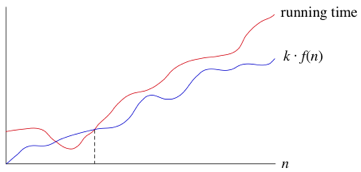
\includegraphics{Omega_fn}
\end{figure}
	\url{https://www.desmos.com/calculator/t8paytwq1w}
\end{frame}

\begin{frame}{Ismétlés --- Aszimptotikus jelölések: $\Theta$}
\begin{figure}
	\centering
	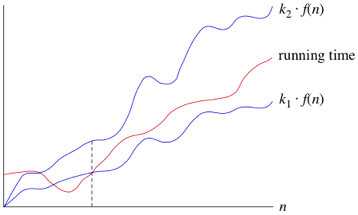
\includegraphics{Theta_fn}
\end{figure}
\end{frame}

\begin{frame}{Ismétlés --- Aszimptotikus jelölések: $O$}
\begin{figure}
	\centering
	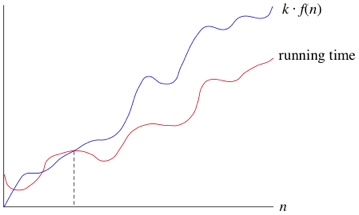
\includegraphics{O_fn}
\end{figure}
\end{frame}

\begin{frame}{Ismétlés -- Aszimptotikus jelölések}
	\begin{alertblock}{\only<2>{(beugratós)} Kérdés}	
		Hatékony-e az az algoritmus, amelyik futási ideje $n$ méretű inputra \textit{legalább} $O(n \log n)$? \\
		\only<2>{Másképp szólva, mit tudunk arról az algoritmusról, amelynek futási ideje $\Omega(1)$?}
	\end{alertblock}
\end{frame}

\begin{frame}{Bináris fa implementációja}
	\begin{itemize}
		\item Egy olyan ''megengedő'' kétszeresen láncolt lista, ahol az elemek (egy helyett) két elemhez is kapcsolódhatnak
	\end{itemize}
	
	\begin{block}{Láncolt lista}
		\begin{tikzpicture}[
		        list/.style={
		            very thick, rectangle split,
		            rectangle split parts=3, draw,
		            rectangle split horizontal, minimum size=18pt,
		            inner sep=5pt, text=black,
		            rectangle split part fill={blue!20, red!20, blue!20}
		        },
		        ->, start chain, very thick
		      ]
		
		  \node[list,on chain] (A) {\nodepart{second} 20};
		  \node[list,on chain] (B) {\nodepart{second} 55};
		  \node[list,on chain] (C) {\nodepart{second} 84};
		
		  \node[squarecross]   (D) [right=of C] {};
		  \node[squarecross]   (E) [left= of A] {};
		
		  \path[*->] let \p1 = (A.three), \p2 = (A.center) in (\x1,\y2) edge [bend left] ($(B.one)+(0,0.2)$);
		  \path[*->] let \p1 = (B.three), \p2 = (B.center) in (\x1,\y2) edge [bend left] ($(C.one)+(0,0.2)$);
		  \draw[*->] let \p1 = (C.three), \p2 = (C.center) in (\x1,\y2) -- (D);
		
		  \draw[*->] ($(A.one)+(0.2,0.1)$) -- (E);
		  \path[*->] ($(B.one)+(0.1,0.1)$) edge [bend left] ($(A.three)+(0,-0.05)$);
		  \path[*->] ($(C.one)+(0.1,0.1)$) edge [bend left] ($(B.three)+(0,-0.05)$);
		\end{tikzpicture}
	\end{block}
\end{frame}

\begin{frame}[fragile]{Bináris fa implementációja}
	\begin{columns}
		\begin{column}{.5\textwidth}
			\begin{lstlisting}[language=c++]
class Node {
    Object kulcs;
    Node* apa;
    Node* bal;
    Node* jobb;
}
			\end{lstlisting}
		\end{column}
		
		\begin{column}{.5\textwidth}
		\begin{figure}
		\centering
\begin{tikzpicture}[node distance=0cm,outer sep = 0pt]
    \node (A) [box,minimum width=6em] {kulcs};
    \node (D) [box,anchor=south,minimum width=6em] at (A.north) {apa};
    \node (B) [box,anchor=north west,minimum width=3em] at (A.south west) {bal};
    \node (C) [box,anchor=north east,minimum width=3em] at (A.south east) {jobb};
    \coordinate (E) at (0,2);
    \coordinate (E) at (0,2);
    \node[below left = 1cm of B] (F) {};
    \node[below right = 1cm of C] (G) {};
%    \path (D) edge [->] node[pos=0.5,anchor=-135,inner sep=1pt] {N} (E);
    \path (D) edge [->] (E);
    \path (B) edge [->] (F);
    \path (C) edge [->] (G);
\end{tikzpicture}
		\end{figure}
		\end{column}
	\end{columns}
\end{frame}

\begin{frame}[fragile]{Fabejárások}
	\begin{itemize}
		\item Inorder/preorder/posztorder bejárások
		\item Legegyszerűbb megvalósításuk rekurzióval történik
		\begin{itemize}
			\item Jó azonban tudni, hogy  \href{https://sites.google.com/site/debforit/efficient-binary-tree-traversal-with-two-pointers}{rekurzió nélkül is megtehető mindez}
		\end{itemize}
	\end{itemize}
	\begin{columns}
		\begin{column}{.3\linewidth}
\begin{alltt}
\small
void \textcolor{green}{in}order(x)\{
  if(x==nil)\{return\}
  inorder(x.bal)
  \textcolor{green}{print(x.kulcs)}
  inorder(x.jobb)
\}
\end{alltt}
		\end{column}
		\begin{column}<2->{.3\linewidth}
\begin{alltt}
\small
void \textcolor{green}{pre}order(x)\{
  if(x==nil)\{return\}
  \textcolor{green}{print(x.kulcs)}
  preorder(x.bal)
  preorder(x.jobb)
\}
\end{alltt}
		\end{column}
		\begin{column}<3>{.3\linewidth}
\begin{alltt}
\small
void \textcolor{green}{post}order(x)\{
  if(x==nil)\{return\}
  postorder(x.bal)
  postorder(x.jobb)
  \textcolor{green}{print(x.kulcs)}
\}
\end{alltt}
		\end{column}
	\end{columns}
\end{frame}

\begin{frame}{Teljes bináris fa}
	\begin{itemize}
		\item Olyan bináris fa, amelynek minden belső csúcsának 2 fia van
	\end{itemize}
	\begin{block}{Fában lévő kulcsok száma}
		A fa $i$-edik szintjén $2^i$ csúcs található \\ \pause $\Rightarrow$ a fában $n=\sum\limits_{i=0}^{h} 2^i=2^{h+1}$ csúcsot található\footnote{bizonyítás teljes indukcióval} \\
		\textbf{Állítás}: $h$ magas fában $O(2^h)$ csúcs található \\ \pause
		\textbf{Megfordítva}: $n$ csúcsból álló fa magassága $\Omega(\log n)$
	\end{block}
\end{frame}

\begin{frame}{Bináris keresőfa}
	\begin{block}{Keresőfa tulajdonság}
		A fa minden $x$ csúcsára teljesül, hogy
		\begin{itemize}
		\item $x.bal.kulcs < x.kulcs$ (amennyiben $x.bal != nil$)
		\item $x.kulcs < x.jobb.kulcs $ (amennyiben $x.jobb != nil$)
		\end{itemize}
	\end{block}
\onslide<2>{
	$<$ rendezés tranzitivitásából adódóan
	\begin{figure}
		\centering
		    \begin{tikzpicture}[level/.style={sibling distance = 2cm, level distance = 1cm}]
		    \node [treenode] {53}
		    child[edge from parent path ={(\tikzparentnode) -- (\tikzchildnode.north)}] {
		            node [subtree] {$<53$}
		        }
		    child[edge from parent path ={(\tikzparentnode) -- (\tikzchildnode.north)}] {
		            node [subtree] {$>53$}
		        }
		    ;
		    \end{tikzpicture}
	\end{figure}
}
\end{frame}

\begin{frame}[fragile]{Kulcs keresése fában}
\begin{columns}
\begin{column}{.5\linewidth}
\begin{alltt}
{\scshape FábanKeres}(x, k) \{
   if x == nil or k == x.kulcs
      return x

   if k < x.kulcs
      {\scshape FábanKeres}(x.bal, k)
   else 
      {\scshape FábanKeres}(x.jobb, k)
 \}
\end{alltt}
\end{column}
\begin{column}<2>{.4\linewidth}
$h$ magas fa esetén $O(h)$
\end{column}
\end{columns}
\end{frame}

\begin{frame}{Elem beszúrása bináris keresőfába}
  \begin{itemize}
    \item A keresőfa tulajdonság fenntartása mellett levélként szúrunk be
	\item $h$ magas fa esetén $O(h)$ idejű
  \end{itemize}
  \begin{example}
 	\begin{figure}
 	    \begin{tikzpicture}
 		    \node[treenode]{20};
 		\end{tikzpicture}
 	\end{figure}

 	{\scshape Beszúr(7)}

	\begin{figure}
		\begin{tikzpicture}
			\node[treenode] {20}
    		child{ node[treenode] {7}}
			child[missing];
 		\end{tikzpicture}
 	\end{figure}
  \end{example}
\end{frame}

\begin{frame}{Elem törlése bináris keresőfából}
\pause
	\begin{itemize}
		\item 3 esetet különböztetünk meg $x$ csúcs törlése kapcsán
		\begin{enumerate}
			\item $x$-nek nincs gyereke
			\begin{itemize}
				\item $x$ apjának az $x$-re vonatkozó mutatóját $nil$-re állítjuk
			\end{itemize}
			\item $x$-nek pontosan egy gyereke van
			\begin{itemize}
				\item $x$ apját ''átkötjük'' $x$ egyedüli fiához
			\end{itemize}
			\item $x$-nek 2 gyereke van
			\begin{itemize}
				\item $x$-et megelőzőjével (bal oldali részfájának maximális elemével) helyettesítjük
			\end{itemize}
		\end{enumerate}
		\item $h$ magas fa esetén $O(h)$ idejű
	\end{itemize}
\end{frame}

\end{document}